\documentclass[a4paper]{article}

\input{Preamble_commands}

\begin{document}

%%%%%%%%%%%%%%%%
% TITLE & NAME %
%%%%%%%%%%%%%%%%
% \selectlanguage{portuguese}  % <-- ACTION: UNCOMMENT for english or portuguese
\selectlanguage{english}  % <-- ACTION: UNCOMMENT for english or portuguese
\title{WebAssembly Distributed Dynamic Inference} % <-- ACTION: WRITE your project title here
\author{André Páscoa} % <-- ACTION: WRITE your complete name here
\istid{110817} % <-- ACTION: WRITE your student number  here (your student number, not the IST-ID)
\email{andre.pascoa@tecnico.ulisboa.pt} % <-- ACTION: WRITE your e-mail here

\advisor{Rodrigo Bruno, Rodrigo Rodrigues}

% To make the title
\maketitle
\thispagestyle{empty}

%%%%%%%%%%%%
% ABSTRACT %
%%%%%%%%%%%%
% To remove indentation before abstract
\setlength{\abstitleskip}{-\absparindent}
\begin{abstract}
% WebAssembly (Wasm) has emerged as a portable compilation target for multiple programming languages, extending beyond its original focus on web applications to domains like cloud computing. Despite its growing adoption, support for AI model inference in Wasm, particularly on serverless platforms like Cloudflare Workers \cite{cloudflareWorkers}, remains limited. The introduction of the WebAssembly Component Model provides a "shared-nothing" abstraction for modules, enabling interoperability between programming languages through memory encapsulation and standardized type specifications (WIT). Within this framework, interfaces like wasi-nn have been proposed to facilitate AI model inference using common backends such as PyTorch\cite{pytorch} and TensorFlow\cite{tensorflow}. However, existing implementations of wasi-nn overlook cost optimization strategies, particularly those related to GPU rental.



The widespread adoption of deep learning models has driven significant technological advancements across domains such as healthcare, developer productivity, data analytics, and education. However, executing inference on infrequently accessed models, such as those hosted on platforms like Hugging Face, presents cost-efficiency challenges. Renting high-performance GPUs, like H100 or RTX 4090, for low-throughput tasks is economically impractical. Existing solutions like DynamoLLM reduce costs by scaling GPU frequency and instances but lack support for heterogeneous vertical scaling.

This work addresses these limitations by proposing a runtime capable of dynamically scaling both vertically and horizontally based on cost-benefit analyses. Our approach improves throughput per dollar by renting cheaper resources, such as RTX 4090 GPUs or CPU VMs, for low-demand inference, while seamlessly scaling to meet production throughput requirements. Implementing this adaptive switching between CPU and GPU inference with existing frameworks like PyTorch requires overcoming challenges related to their distinct shared libraries and model weights management.

By incorporating cost-benefit analysis, our runtime will support vertical scaling—switching between GPU types, such as from an RTX 4090 for testing to an H100 for production—alongside horizontal scaling. This approach provides cost-efficient deployment options, from initial testing to production, and seamlessly integrates with existing Wasm applications via the standardized WebAssembly Component Model.

% \keywords{Keyword 1, Keyword 2, Keyword 3} % <--- ACTION: WRITE YOUR KEYWORDS HERE
\clearpage
\end{abstract}

%%%%%%%%%%%%%%%%%%%%%
% TABLE OF CONTENTS %
%%%%%%%%%%%%%%%%%%%%%
\tableofcontents
\thispagestyle{empty}
\clearpage


%% <-- ACTION: ADD/EDIT/REMOVE/COMMENT SECTIONS IF YOU NEED TO
%%%%%%%%%%%%%%%%
% INTRODUCTION %
%%%%%%%%%%%%%%%%

\section{Introduction}

The exponential growth in the adoption of deep learning models has positioned them at the core of numerous technological advancements and applications. These models are now employed across various domains, including healthcare, developer productivity, data analytics, education, and beyond. When accessing infrequently accessed models however, like those hosted on platforms such as Hugging Face, renting an entire H100 or even an RTX 4090, which have high rental costs, for such low-throughput, is not cost-effective.

Existing work such as DynamoLLM \cite{dynamollm} achieves 61\% reduced operational costs by configuring GPU frequency and the number of instances for running a model based on the incoming request token distribution. This however, does not take into the opportunity of heteregenous vertical scaling, and only does horizontal scaling by changing the number of instances. By renting a cheaper GPU such as an RTX 4090 or possibly a CPU VM when executing few inference invocations, throughput per unitary cost should improve.

This allows for more flexibility where if we want to do inference of some LLM for testing initially, our solution rents a cheap GPU or CPU, but when deploying in production it automatically vertically and horizontally scales to meet the new throughput requirements.

However, to implement this switching between a GPU or a CPU for inference with software such as PyTorch is not trivial. Due to the way PyTorch binaries are packaged, which contain separate shared libraries for CPU and GPU processing, we need to create an abstraction that enables interfacing with both these shared libraries and also do the switching of the model weights between them.

WebAssembly (Wasm) is a new technology that has brought a portable compilation target for various programming languages. Originally meant for the web, it has now expanded to other domains such as cloud computing.

Furthermore, with the arrival of the WebAssembly Component Model which aims to bring a shared-nothing abstraction for Wasm modules enabled due to memory encapsulation in each component, interoperability between different programming languages compiled to WebAssembly with an immutable type specification (WIT) is now possible.

% With the arrival of the WebAssembly Component Model which aims to bring a shared-nothing abstraction for wasm modules enabled due to memory encapsulation in each component that enables interoperability between different programming languages with a standardized type specification (WIT), new interfaces have been proposed. 
% One of these interface proposals is \textit{wasi-nn} which allows doing model inference with a common backend such as PyTorch\cite{pytorch} or Tensorflow\cite{tensorflow}

% \item Why is it hard? (E.g., why do naive approaches fail?)

% The use of WebAssembly as a common layer across the cloud-edge continuum has been explored by Ménétrey et al. \cite{menetrey2022webassembly}, who highlight how WebAssembly can bridge the gap between proprietary silos across cloud, edge, and IoT devices, while maintaining strong performance. To verify that WebAssembly is able to achieve strong performance compared to native and across the cloud-edge continuum, they ran benchmarks on a x86 intel cloud server and an arm edge processor. These benchmarks consisted of the PolyBench/C Benchmarks and benchmarking a WebAssembly compiled version of SQLLite. These show that the slowdown relative to the native version varied from 1.3X on the PolyBench/C Benchmarks and at maximum 2.7x in the x86 processor, the performance also has improved over time, with previous versions of the WAMR runtime they used in 2020 having considerable worse performance (4.1x slowdown compared to the native architecture). They also show that security guarantees of the execution of the applications can be achieved despite running these applications on untrusted edge hardware, by using Trusted Execution Environments (TEEs), such as Intel SGX and Arm TrustZone.

% Existing WebAssembly modules outside the web are mostly static and do not support dynamic linking. Even if loaded dynamically, these modules are still assumed to be loaded locally. We introduce a custom runtime that is able to run WebAssembly modules in a distributed environment, where modules can be loaded and function calls executed remotely. 

% Currently the support for AI model inference with WebAssembly is limited, and serverless platforms such as Cloudflare Workers \cite{cloudflareWorkers}, do not currently support AI model inference. 



% Service Weaver\cite{ghemawat2023towards} proposes a new framework that allows developers to build a logical monolith that is then split into microservices and distributed by the framework runtime. This allows the runtime to make choices regarding co-location of microservices to increase performance or to run the logical monolith in the same process to simplify integration tests. Blueprint\cite{anand2023blueprint} proposes a framework that simplifies microservice deployment by providing a toolchain that allows easy reconfiguration of the microservices, such as switching between RPC libraries or adding logging. Both of these solutions simplify the deployment and reconfiguration of microservices, but they are not seamless and require the developer to use their framework.


% \item What is the problem?


% \item Why hasn't it been solved before? (Or, what's wrong with previous proposed solutions? How does mine differ?)
% \item What are the key components of my approach and results? Also include any specific limitations.

% However, dynamic linking of WebAssembly modules is still in its infancy. Currently, both the Emscripten and \texttt{wasi-sdk} toolchains enable the creation of shared library module. Emscripten also allows load-time linking and runtime linking with \texttt{dlopen}, while \texttt{wasi-sdk} does not. However, there are tools for WASI version 2, such as \texttt{wasm-tools component link} and \texttt{componentize-py}, that do include load time linking and runtime linking by implementing the \texttt{dlopen}/\texttt{dlsym} symbols.

% WASI version 2 is still a Phase 1 WebAssembly \href{https://github.com/WebAssembly/proposals}{proposal} and not yet standardized, and Emscripten does not implement the full WASI standard. Thus, we chose to implement our own runtime based on \href{https://helda.helsinki.fi/bitstream/10138/335259/1/WAsDE_SAC2021.pdf}{Mäkitalo, Niko et al}. \href{https://helda.helsinki.fi/bitstream/10138/335259/1/WAsDE_SAC2021.pdf}{Mäkitalo, Niko et al} use Wasmtime as a base runtime and implement dynamic linking by parsing the \texttt{dylink.0} \href{https://github.com/WebAssembly/tool-conventions/blob/main/DynamicLinking.md}{custom section} of the shared libraries. This custom section contains the information required to determine the shared library's dependencies, memory and function table requirements, and load them at runtime with the standard \texttt{dlopen}/\texttt{dlsym} functions.

% Serverless computing has been a popular topic in recent years. While current solutions such as Firecracker micro VMs have high tail latencies due to the need to recreate runtimes for each function, newer solutions such as Dandelion propose a new programming model that separates compute and IO functions. This programming model increases isolation and thus allows for reusing the runtime, which reduces the cold start latency. Another approach is Palette Load Balancing, which allows the developer to specify locality hints so that state can be cached across invocations. These hints enable the load balancer to redirect the same invocations to the same servers and thus increase cache usage. For a serverless web application with a local cache, Palette improves the hit ratio by 6x.



We thus propose a runtime that dynamically does this vertical and horizontal scaling based on a cost-benefit analysis, which is easily extended into existing WebAssembly applications due to the use of the standardized WebAssembly Component Model. 

\subsection{Contributions}

Our work introduces the following key contributions:

\begin{enumerate}
    \item \textbf{Vertical Scaling}
    
    By scaling from cheap CPU VMs to more expensive GPUs based on throughput, we obtain greater cost-benefit than existing work focused only on GPU orchestration such as DynamoLLM \cite{dynamollm}.
    
    \item \textbf{Standardized WebAssembly-Based Architecture} 
    
    Our solution provides an inference framework that leverages WebAssembly’s Component Model for interoperability across programming languages, simplified microservices due to wRPC and portability due to WebAssembly itself. 

    \item \textbf{WebAssembly LibTorch Wrappers}
    
    We implement a custom runtime with a WebAssembly component model wrappers for the CPU and GPU LibTorch libraries to access it from other components.

\end{enumerate}

\subsection{Document Outline}

The remainder of this work assumes the following structure:

\begin{itemize}    
    \item \textbf{Section 2: Background} Provides a technical background in WebAssembly, which is one of the key components of our solution.

    \item \textbf{Section 3: Related Work} Reviews notable contributions in
WebAssembly enhancements regarding dynamic linking, energy optimization in large-scale training and inference systems.

    \item \textbf{Section 4: Solution} Describes the dynamic resource selection, architecture, and implementation details of our proposed framework.

    \item \textbf{Section 5: Evaluation} Discusses the research hypothesis, expected results, chosen metrics, evaluation environment and workload.

    \item \textbf{Section 6: Work Schedule} Outlines our proposed work schedule.
\end{itemize}


\pagebreak

% For advice on how to write and structure a paper, see the following link (some of the content in this template is taken from this link):

% \url{https://cs.stanford.edu/people/widom/paper-writing.html?s=03#intro}

% \medskip

% Read and bookmark the page above. You are recommended to follow the ``Stanford InfoLab's patented five-point structure for Introductions''. Unless there's a good argument against it, the Introduction should consist of five paragraphs answering the following five questions:

% \begin{enumerate}
% \item What is the problem?
% \item Why is it interesting and important?
% \item Why is it hard? (E.g., why do naive approaches fail?)
% \item Why hasn't it been solved before? (Or, what's wrong with previous proposed solutions? How does mine differ?)
% \item What are the key components of my approach and results? Also include any specific limitations.
% \end{enumerate}

% \paragraph{\textbf{A few notes on the use of \LaTeX.}} 
% First, double quotes are done with \verb|``| and \verb|''|. For example, \verb|``double quotes''| yields ``double quotes''. Note that if you write \verb|"double quotes"|, you obtain "double quotes" (which doesn't look as nice).

% Citations are done with the \verb@\cite@ command \cite{Goodfellow:2014}. 
% Note that it is always preferable to be possible to read your text without the references. For example, sentences like the following should be avoided:

% \begin{quote}
% \sl
% Generative adversarial networks were first introduced in \cite{Goodfellow:2014}.
% \end{quote}
% Instead, one can write:
% \begin{quote}
% \sl
% Goodfellow et al. introduced and described Generative adversarial networks~\cite{Goodfellow:2014}.
% \end{quote}

 
% Bibliographic entries are placed in the file \textsf{Bibliography.bib}.
% This is another citation \cite{McDonagh:2011dp} and this is another one \cite{Feller:2011ys}.
% \textbf{Important:} in most cases, you do not need to create the bibliographic entry manually; instead, you can use a service like Google Scholar\footnote{Extracting bibtex entries from Google Scholar: \url{https://libguides.usask.ca/c.php?g=218034&p=1445751}}, which is recommended for you to find related work.

% For advice on creating professional and clean tables with \LaTeX, see:

% \url{https://texblog.org/2017/02/06/proper-tables-with-latex/}

% Table~\ref{tab:example} is an example.

% \subsection{Work Objectives}
% \lipsum[2] % remove this

% \subsection{Expected Contributions}
% \lipsum[2] % remove this



%%%%%%%%%%%%%%
% Background %
%%%%%%%%%%%%%%

% \section{Background} 
% \subsection{Subsection 1}
% \lipsum[10]
% \begin{enumerate}
%     \item Point 1
%     \item Point 2
%     \item Point 3
% \end{enumerate}
% \lipsum[1]

\section{Background}

In this section, we provide a technical background in WebAssembly, which is one of the key components of our solution. This technology appeared as consequence of the rapid evolution of software development, which introduced microservices as a dominant architectural paradigm, offering modularity, scalability, and improved resource optimization. Modern frameworks and technologies have emerged to address the challenges of orchestrating microservices effectively, including communication, performance tuning, and seamless deployment. Among these, WebAssembly (Wasm) has gained prominence as a portable and efficient runtime that bridges the gap between cloud and edge environments. This section explores notable microservice frameworks, the capabilities of WebAssembly, and its role as a unifying layer across diverse infrastructures.

\subsection{Microservice Frameworks}
Modern microservice frameworks, such as Service Weaver\cite{ghemawat2023towards} and Blueprint\cite{anand2023blueprint} simplify the challenges of microservice orchestration, such as communication, performance optimization, and reconfiguration.

Microservice frameworks provide a structured and organized approach to building, deploying, and managing microservices. These frameworks simplify the complex processes associated with microservice architecture, enabling developers to focus more on business logic rather than the intricacies of infrastructure. 

This decomposition allows optimization of existing resources, such as colocation of business logic modules. We take this into consideration when choosing our technology stack, the WebAssembly Stack, which standardizes decomposition with the WebAssembly Component Model.

Below, we discuss the two notable frameworks, Blueprint\cite{anand2023blueprint} and Service Weaver\cite{ghemawat2023towards}, which offer distinct features but present the same principal drawback.

\subsubsection{Blueprint Framework}
Blueprint\cite{anand2023blueprint} proposes a solution that simplifies microservice deployment by providing a toolchain to automatically build and deploy microservices. The framework generates code based on two key specifications:

\begin{itemize}
    \item \textbf{Workflow Specifications}: Defines the business logic of the application, which can be seen in Figure \ref{fig:workflow-spec}.
    \item \textbf{Wiring Specifications}: Details the scaffolding, including component interactions, logging, and RPC library integration. This code can be seen in figure \ref{fig:wiring-spec}
\end{itemize}

\begin{figure}[h!]
\centering
\begin{minipage}{0.48\textwidth}
    \centering
    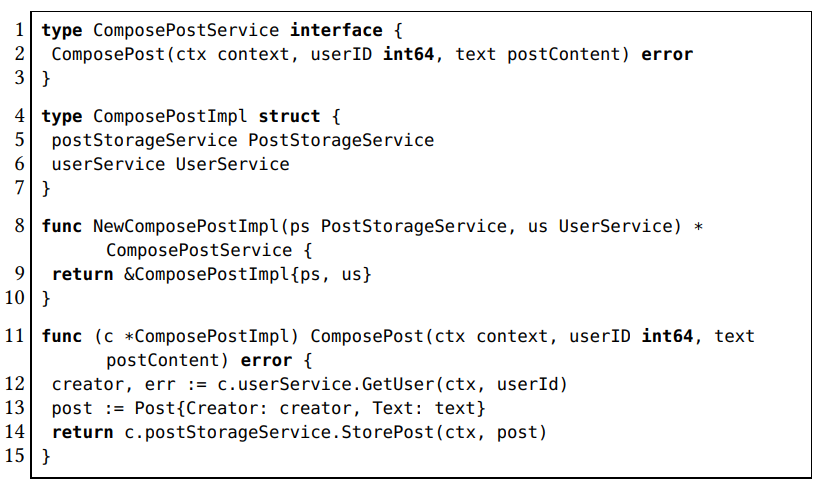
\includegraphics[width=\textwidth]{Images/workflow_spec.png}
    \caption{Workflow specification for defining business logic.}
    \label{fig:workflow-spec}
\end{minipage}
\hfill
\begin{minipage}{0.48\textwidth}
    \centering
    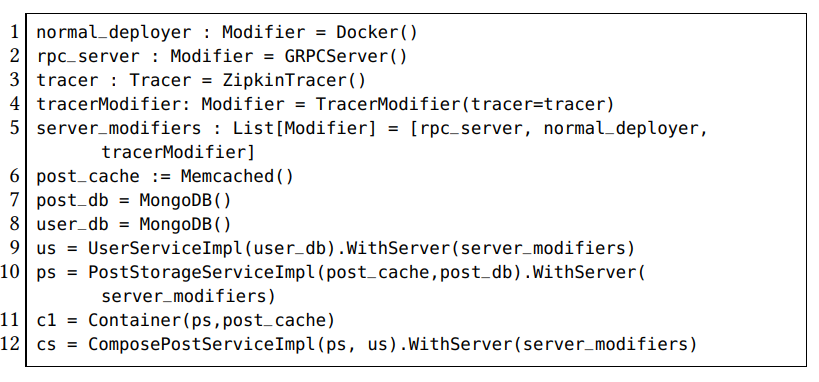
\includegraphics[width=\textwidth]{Images/wiring_spec.png}
    \caption{Wiring specification detailing the microservices scaffolding.}
    \label{fig:wiring-spec}
\end{minipage}
\end{figure}

This architecture allows for easier reconfiguration; for instance, switching between RPC libraries or adding logging typically requires only 1-5 lines of changes in the wiring specifications.

While Blueprint significantly reduces the complexity of microservice management, it is not entirely seamless and mandates developers to work within its framework.

\subsubsection{Service Weaver Framework}
Service Weaver\cite{ghemawat2023towards} addresses five challenges of microservices: performance degradation, correctness issues, management complexity, API versioning constraints, and slowed application development. To resolve these issues, Service Weaver introduces a framework that enables:

\begin{itemize}
    \item \textbf{Service Co-location}: Enables function calls to operate locally, or as remote RPCs based on runtime decisions.
    \item \textbf{Simplified Microservice Testing}: Integration testing is simplified, because local modes can function effectively as unit tests without requiring remote calls.
    \item \textbf{API Versioning}: Mitigates API versioning problems due to updates to the application code being applied holistically.
\end{itemize}

While having multiple advantages, Service Weaver \cite{ghemawat2023towards} also requires developers to adopt its specific framework, limiting developer experience.

\subsection{WebAssembly (Wasm)}
WebAssembly (Wasm) is a portable, low-level binary instruction format designed to serve as a compilation target for various programming languages, such as C, C++, and Rust. Initially created for the web, Wasm has become a transformative technology that now spans across domains like cloud computing, edge computing, IoT, and even serverless architectures.

Wasm allows developers to write applications in their preferred languages and compile them into an intermediate format that is both efficient and portable. Its architecture provides near-native execution speed while maintaining strong security guarantees, making it ideal for performance-critical applications.

Key advantages of Wasm include:
\begin{itemize}
\item \textbf{Portability}: Wasm binaries can run on any platform equipped with a browser or other runtime that supports Wasm.
\item \textbf{Efficiency}: Wasm provides low-latency execution with fast startup times, useful for cloud and edge workloads.
\item \textbf{Isolation}: Applications run securely within a sandboxed environment, reducing risks of unauthorized access or corruption.
\end{itemize}

In addition to its primary role in web applications, Wasm is increasingly being adopted in edge computing scenarios, where its efficiency and portability allow developers to deploy lightweight containers on low-resource devices.

\subsection{WebAssembly System Interface (WASI)}
The WebAssembly System Interface (WASI) extends WebAssembly's capabilities beyond the browser, enabling interaction with system resources. It provides a set of APIs for operating system functionalities, such as file I/O, network sockets, clocks, and process management.

WASI ensures that Wasm modules can run across different platforms, from edge devices to large cloud servers, without requiring changes to the application code.

Currently, WASI is available in two versions:
\begin{itemize}
\item \textbf{WASI v1}: A foundational system interface supporting essential features like file access and most system calls.
\item \textbf{WASI v2}: Introduces a component model that enables modular, reusable, and interoperable WebAssembly components. This model facilitates better integration between different programming languages and tools with a common interface (WIT).
\end{itemize}

\subsection{The Component Model}
The Component Model, introduced in WASI v2, is a significant advancement in WebAssembly's modular ecosystem. It provides a higher-level abstraction for Wasm modules, allowing dynamic linking and safe interaction between components.

With a \textbf{shared-nothing} architecture, components interact through explicit interfaces. This ensures strong isolation while enabling clean communication. Key features of the Component Model include:
\begin{itemize}
\item \textbf{Dynamic Linking}: Unlike WASI v1 which does not support \textbf{dlopen} nor \textbf{dlsym} (which are explained in Section \ref{sec-3.1}), modules inside a component can be loaded at runtime.
\item \textbf{Interoperability}: Components written in different languages communicate via standardized WIT interfaces.
\item \textbf{Memory Encapsulation}: Each module manages its linear memory, ensuring no unintended sharing of resources.
\end{itemize}

\subsection{WebAssembly Interface Types (WIT)}
The WebAssembly Interface Types (WIT) specification simplifies interoperability between modules written in different programming languages. Traditionally, WebAssembly modules used low-level types like integers and pointers, which made sharing complex data structures across modules difficult.

WIT introduces high-level types such as strings, lists, and records, allowing modules to communicate seamlessly. It serves as a bridge, enabling components written in Rust, Go, or C++ to interact without needing extensive type conversions or manual serialization.

Key contributions of WIT include:
\begin{itemize}
\item \textbf{Simplified Communication}: Abstracts low-level complexities to enable clear and structured module interactions.
\item \textbf{Immutable Interface}: Due to the immutable interface, which is enforced by the component model's shared nothing architecture, where each component has its own linear memory, components may be distributed.
\item \textbf{Language Agnosticism}: Promotes modular development across multiple programming languages with shared types.
\item \textbf{Type Safety}: Reduces errors by ensuring consistency in data representation.
\end{itemize}

\subsection{WebAssembly RPC (wRPC)}
WebAssembly RPC (wRPC) is a protocol that facilitates Remote Procedure Calls (RPC) between Wasm modules. By using Wasm's component model architecture, wRPC enables distributed communication across environments, such as edge servers and cloud infrastructure.

This approach abstracts the complexities of component interaction and allows function calls between remote Wasm components to appear as local operations. wRPC enhances scalability by enabling distributed execution while preserving Wasm's strong isolation guarantees.

The \textbf{wRPC protocol} is a transport-agnostic system designed for asynchronous communication of WebAssembly Interface Types (WIT) function calls within a client-server architecture. Supporting multiplexed, bidirectional data streams, it utilizes the component model value definition encoding for serialization.

\subsubsection*{Key Features}
\begin{itemize}
\item \textbf{Transport Protocols}: Compatible with TCP, QUIC, Unix Domain Sockets, and NATS.io, among others.
\item \textbf{Multiplexing}: Supports concurrent handling of multiple data streams, enabling efficient execution of asynchronous functions such as input/output streams.
\item \textbf{Encoding}: Implements the component model's value encoding, extended for streams ($list$).
\end{itemize}

\subsubsection*{Framing Specification}
Messages in wRPC start with a version byte and a \texttt{header} structure, followed by frames containing indexed paths and data payloads, which:

\begin{itemize}
\item Facilitates resource-efficient RPC calls.
\item Offers modularity across various transport mechanisms.
\item Seamlessly integrates with WebAssembly's component model.
\end{itemize}

This makes wRPC a good choice for high-performance distributed systems and WebAssembly applications requiring remote module execution such as our work.

\subsection{WebAssembly as a common layer across the cloud-edge continuum}

The use of WebAssembly as a common layer across the cloud-edge continuum has been explored by
Ménétrey et al \cite{menetrey2022webassembly}, who highlight how WebAssembly can bridge the gap between proprietary silos across
cloud, edge, and IoT devices, while maintaining strong performance. 

To verify that WebAssembly is
able to achieve strong performance compared to native and across the cloud-edge continuum, they run
benchmarks on a x86 intel cloud server and an arm edge processor. These benchmarks consist of
the PolyBench/C Benchmarks and benchmarking a WebAssembly compiled version of SQLLite.
These show that the slowdown relative to the native version varied from 1.3X on the PolyBench/C Benchmarks
and at maximum 2.7x in the x86 processor, the performance also has improved over time, with previous
versions of the WAMR runtime they used in 2020 having considerable worse performance (4.1x slowdown
compared to the native architecture). 

They also show that security guarantees of the execution of the applications can be achieved despite running these applications on untrusted edge hardware, by using
Trusted Execution Environments (TEEs), such as Intel SGX and Arm TrustZone.

% Consider Table~\ref{tab:example} below.
%% For tables, see:
% - https://jdhao.github.io/2019/08/27/latex_table_with_booktabs/
% - https://people.inf.ethz.ch/markusp/teaching/guides/guide-tables.pdf
% \begin{table}
%     \centering
%     \caption{Description}
%     \label{tab:example}
%     \begin{tabular}{@{}lllll@{}}
%         \toprule
%         \multirow{2}{*}[-1em]{Models} & \multicolumn{3}{c}{Metric 1} & Metric 2\\
%         \addlinespace[10pt]
%         \cmidrule(lr){2-4} \cmidrule(lr){5-5} \\
%         {} & precision & recall & F-score  & R@10 \\
%         \midrule
%         model 1 & 0.67  & 0.8 & 0.729  & 0.75 \\
%         model 2 & 0.8 & 0.9 & 0.847 & 0.85 \\
%         \bottomrule
%     \end{tabular}
% \end{table}



%%%%%%%%%%%%%%%%
% Related work %
%%%%%%%%%%%%%%%%
\section{Related Work}

Recent advancements in cloud computing, WebAssembly, and energy-efficient frameworks have sparked numerous innovations in system design and optimization. This section reviews notable contributions in WebAssembly enhancements, energy optimization in large-scale training and inference systems. These works highlight the state-of-the-art methodologies and provide a foundation for our proposed approach.

% \subsection{Function as a Function}

% Function as a Function \cite{kuchler2023function} propose dandelion, a FaaS system that adds a new programming paradigm where functions are divided into compute and IO functions. Developers create the compute functions and agglomerate them with IO functions into what they call compositions. This programming model makes it easier to achieve isolation and thus runtimes do not need to be recreated like in the Firecracker micro VM. This achieves 45x lower tail latency (latency of the highest latency requests) for cold starts.

% As with the microservice frameworks Service Weaver and Blueprint, this work is not seamless and is dependent on a new framework.

% With the arrival of WebAssembly however, since it already provides a trusted system interface (WASI), there’s no need for this programming model of separating IO and compute.

\subsection{Bringing WebAssembly Up to Speed with Dynamic Linking}
\label{sec-3.1}

Recent advances in WebAssembly (Wasm) have expanded its applicability beyond web applications to include cloud computing, edge devices, and distributed systems. However, its lack of built-in support for dynamic linking presents significant challenges when designing modular and efficient distributed applications. Addressing this gap, the work by Makitalo et al. \cite{makitalo2021bringing} develops a custom runtime based on WasmTime that extends its capabilities to implement dynamic linking.

In their approach, they parse the dylink.0 custom section of shared library WebAssembly modules.
This section encodes metadata, including:

\begin{itemize}
\item Shared library dependencies,
\item Memory size and alignment requirements,
\item Function table requirements.
\end{itemize}

Using this metadata, the authors implement the \textit{\textbf{dlopen}} and \textit{\textbf{dlsym}} functions, which are not natively supported in WASI v1. These functions enable runtime linking of shared libraries.

We build upon this work as the basis for our initial solution proposal to enable remote module execution.


% \begin{figure}[h!]
% \centering
% 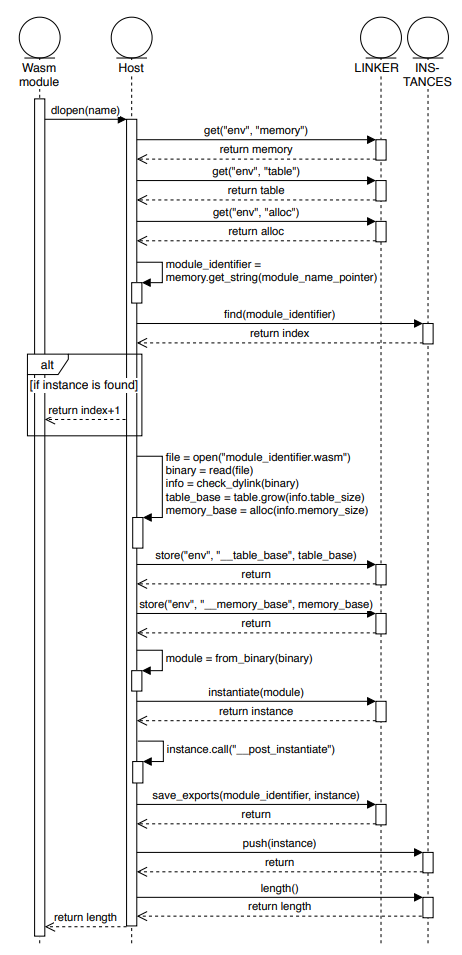
\includegraphics[width=0.5\textwidth]{Images/dynamic-linking-flow.png}
% \caption{Sequence diagram of the \textit{\textbf{dlopen}} function call by Makitalo et al. \cite{makitalo2021bringing}}
% \label{fig:dynamic-linking-flow}
% \end{figure}

\subsection {Reducing Energy Bloat in Large Model Training
}

Training large AI models on numerous GPUs consumes a massive amount of energy, making power delivery one of the largest limiting factors in building and operating datacenters for AI workloads. However, as demonstrated by the work on Perseus \cite{chung2024reducing}, not all energy consumed during training directly contributes to end-to-end throughput. A significant portion can be removed without slowing down training. This portion is referred to as energy bloat.

The work on Perseus addresses this issue by identifying two independent sources of energy bloat in large model training and proposing a training system to mitigate both by slowing down the frequencies of the individual Streaming MultiProcessors in Nvidia GPUs.

One possible cost optimization we could include in our work would be to downsize the hardware when the frequency achieves a certain threshold, but it is not clear whether this would bring any benefit due to the high-bandwidth mesh that is used for these clusters. This work is also focused on training as opposed to our work on inference.

\subsection {DynamoLLM: Designing LLM Inference Clusters
for Performance and Energy Efficiency}

The paper introduces DynamoLLM\cite{dynamollm}, an energy-management framework for Large Language Model (LLM) inference clusters. DynamoLLM\cite{dynamollm} aims to optimize the energy efficiency and cost of LLM serving while meeting Service Level Objectives (SLOs) such as latency constraints, to do this they exploit the \textbf{heterogeneity} and \textbf{fluctuations} in the inference workloads.

This \textbf{heterogeneity} can be found in the computational phases of LLMs, where first, in the prefill phase, input tokens are computed in parallel, and, in the second phase, the decode phase, the LLM autoregressively generates the output tokens. Since the number of output tokens is not known at request time, they predict this number. One example of an optimization they do is that they then use the input and output token length and select the appropriate pool with the correct model parallelism and gpu frequency configuration based on energy consumption historical data. One example of a energy consumption profile for a Llama2-70B can be seen in Figure \ref{fig:dynamo-llm}.

\begin{figure}[h!]
\centering
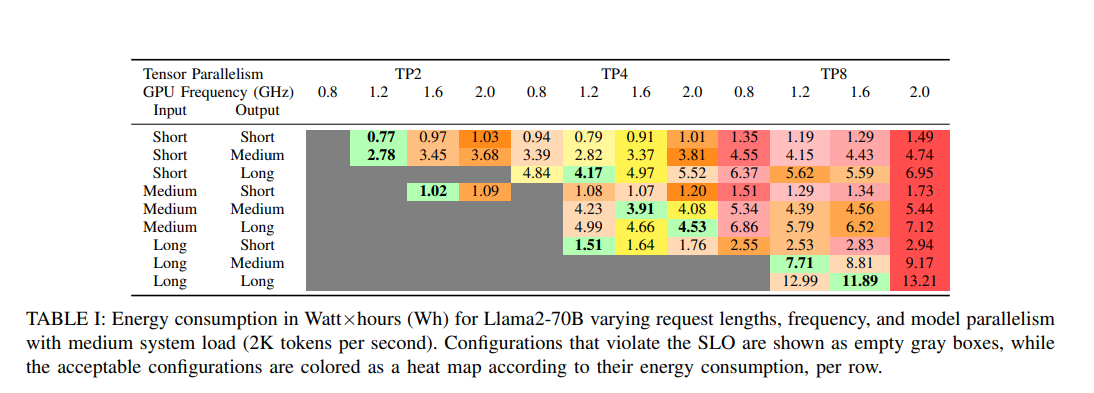
\includegraphics[width=1.0\textwidth]{Images/dynamo-llm.png}
\caption{Dynamo-LLM\cite{dynamollm} Energy Consumption with varying input and output tokens.}
\label{fig:dynamo-llm}
\end{figure}

\subsubsection*{DynamoLLM Framework}
Some of the key features of this framework include:
\begin{enumerate}
    \item \textbf{Instance Reconfiguration:} Dynamically adjusts the number of instances, GPU frequency, and model parallelism.
    \item \textbf{Hierarchical Controllers:} Divides control tasks across cluster, pool, and instance levels.
    \item \textbf{Predictive Scheduling:} Predicts request types, such as output token length and adjusts resource allocation accordingly.
\end{enumerate}

\subsubsection*{Evaluation}

The framework was evaluated on a large-scale GPU cluster using production-level workloads with the following results:

\begin{itemize}
    \item \textbf{Energy Savings:} DynamoLLM conserves 53\% energy compared to traditional setups.
    \item \textbf{Carbon Emission Reduction:} Achieves a 38\% reduction in operational carbon emissions.
    \item \textbf{Cost Efficiency:} Reduces operational costs by 61\% while meeting latency requirements (SLOs)
\end{itemize}

One possible downside this work might have is possibly having fixed hardware type for the pools, since the code is not provided, there's no guarantee, but based on the evaluation they've done (only H100's), it might not support true downscaling to cheaper GPU's and possibly CPU VM's with vertical scaling as our work does.

\subsection{Discussion}

The reviewed works address specific challenges in their respective domains, but gaps remain that our proposal targets.

The work by Makitalo et al. extends WebAssembly with dynamic linking, enabling runtime library loading via \textit{dlopen} and \textit{dlsym}, and we use its ideas for our initial remote module execution proposal.

Perseus optimizes GPU frequency management to reduce energy consumption during large-scale model training. Although effective for training, it does not address inference-specific requirements. Our work extends dynamic resource allocation to heterogeneous hardware, focusing on inference workloads and enabling cost-efficient scaling.

DynamoLLM improves energy efficiency and performance for LLM inference clusters through workload-specific optimizations. However, its design seems to not allow vertical scaling, only horizontal scaling via adding more instances, this limits its applicability to lower-cost hardware configurations. Our proposal supports both vertical and horizontal scaling and integrates WebAssembly for extensibility and portable execution across cloud and edge environments.

%%%%%%%%%%%%
% Solution %
%%%%%%%%%%%%



\section{Solution}
\label{solution}

Our solution to improve throughput per unitary cost when doing model inference first starts by being able to dynamically choose between different types of hardware with a variance of unitary cost per hour, for this we show an initial simplified version that only selects between a CPU VM and one type of rented GPU, but this should easily be expanded to a bigger variety of hardware accelerators. When doing inference however, to easily switch between the accelerators without shutting down the microservice running the code, we choose to run the main application code separate from the model inference on the hardware accelerator, and thus we require a way to link the our interface to a possibly local execution in the case of CPU inference, or remote execution for GPU inference.


\subsection{Dynamic Module Selection}

To optimize throughput per unitary cost, we select different hardware accelerators based on current throughput and utilization characteristics.

\subsubsection{High Throughput and High Device Utilization (HDU)}

When the system operates at high throughput and thus high device utilization (HDU), GPUs should generally the optimal choice. GPUs should provide at high device utilization superior throughput per unitary cost and per watt (W) due to their parallel processing capabilities and the inherent parallelizability of deep learning model inference and training.
This makes them always suitable for training models, where high device utilization is a common scenario.

\subsubsection{Low Throughput and Low Device Utilization (LDU)}

In contrast, low throughput and low device utilization (LDU) may be encountered during inference, especially for rarely accessed models like those hosted on platforms such as Hugging Face. In these scenarios, CPUs emerge as the more cost-effective option. CPUs should offer better throughput per unitary cost in LDU conditions because they consume less power when idle or underutilized, and their energy requirements do not scale as drastically as GPUs.

Considering energy consumption from a holistic perspective\textemdash{}factoring in the energy used by the orchestrator or main CPU server in addition to the GPU\textemdash{}CPUs may also demonstrate higher throughput per watt. This is particularly true in architectures where separate servers are used for orchestration and computation. 

To implement this we obtain throughput per unitary cost profiles of each of the possible hardware types from a historical throughput profiles data source and select the lowest unitary cost for our current inference throughput, we outline the final architecture for this dynamic selection in section \ref{optimized-solution}.


 As we discussed in section \ref{solution}, our solution separates the inference hardware accelerators from the main microservice component to prevent it from being shutdown, thus we require a way to link these the main microservice component with the inference hardware accelerator components, to do this we propose an initial solution based on dynamic linking with WebAssembly primitives, and then improve on this initial proposal's performance bottlenecks by using modern WebAssembly component model infrastructure.

\subsection{Remote Module Execution with Dynamic Linking}
Our initial solution for remote module execution uses WASI v1 and Wasmtime runtime abstractions, such as \textbf{Store}, \textbf{Linker}, and \textbf{Module}, to implement dynamic linking. This involves manually handling shared libraries, memory, and tables.

Before implementing remote module execution, first we require a dynamic linking implementation for linking modules since WASI v1 does not implement this.

% Dynamic linking steps:

% 1 - Create Store and Linker 
% 2 - populate linker with (dlopen, dlsym, dlerror)
% 3 - if required table and memory is created and store references in linker
% 4- read dylink section of main module, extract shared library dependencies and for each shared library do step 4 through 7.
% 5 - Extract from current module dylink section memory size, memory alignment, table size, and table requirements alignment, expand memory and table accordingly.
% 5 - read share library dependencies, execute step 4 recursively.
% 6 - Instantiate current module with linker, which resolves all imports automatically.
% 7 - Obtain exports from the instantiated module and place their references in linker.
% 8 - Now get the main instantiated module and call it's entry function

\subsubsection{Application Compilation}
To create these modules, we use the WASI SDK compiler toolchain with -fPIC, -shared and -Wl,--export-all flags to compile our shared libraries.
%TODO: Why is position independent code required for the shared library? What happens if the flag is not set? Explain%
The -fPIC Flag makes sure the compiler generates position independent WASM code, the -shared flag generates the shared library and the -Wl,--export-all flag makes sure the linker exports all symbols even if unused. After compiling the shared libraries, we use also compile the main module as a shared library.

\subsubsection {Dynamic Linking Approaches}
There are multiple approaches to dynamic linking, such as shared-nothing dynamic linking, shared-something dynamic linking, and shared-everything dynamic linking.

\subsubsection{Shared-Nothing Dynamic Linking}

Shared-nothing dynamic linking architecture is an approach to dynamic linking that does not allow for the sharing of resources between modules other than with explicit communication. This approach is used in the Component Model, which is a part of the WebAssembly System Interface (WASI) v2 standard. The Component Model is an abstraction above WebAssembly modules that allows communication between components of two different languages. It adds common types for lists, strings, etc., which differ between languages to enable this communication. The Components Model forces the developer to specify an interface (thus the explicit communication) that only contain immutable copied values, opaque typed handles and immutable uninstantiated modules, and also fully encapsulates linear memories, tables and globals, thus it does not allow for shared resources between modules.

The main advantage of shared-nothing dynamic linking is that it provides strong isolation between modules, modules cannot accidently or maliciously access each other's resources. However, this isolation comes at the cost of performance, as it requires explicit communication between modules to share resources and can lead to increased memory usage due to the duplication of resources.

\subsubsection{Shared-Everything Dynamic Linking}

Shared-everything dynamic linking architecture is an approach to dynamic linking that allows for the sharing of all resources between modules. This includes the function table, memory, and global variables. This approach is used in the WebAssembly dynamic linking proposal, which is a part of the WebAssembly System Interface (WASI) standard. The proposal defines a new section in the WebAssembly binary format called `dylink.0` that contains the information required to determine the shared library's dependencies, memory and function table requirements, and load them at runtime with the standard `dlopen`/`dlsym` functions.


\subsubsection{Dynamic Linking Implementation}

We base our dynamic linking implementation on existing work \cite{makitalo2021bringing} that was done for the EMScripten compiler toolchain and not the WASI SDK compiler toolchain. This work focused on runtime dynamic linking with dlopen, dlsym, dlerror symbols, while ours will be focused on load time dynamic linking.

As a base we use the WASMTime runtime API in Rust, which gives use abstractions for WebAssembly objects such as Table, Memory, Module, Instance, and also other relevant abstractions such as a Linker for linking imports and exports of multiple module or Store, which stores references to instances, functions, etc..

To implement load time dynamic linking, we start by creating the Store and Linker objects. After that we create Table and Memory objects and store their references in the linker. To know what shared library dependencies the main module requires, we read the dylink.0 section of the WASM Binary and extract them from the WASM\_DYLINK\_NEEDED subsection as specified in the \href{https://github.com/WebAssembly/tool-conventions/blob/main/DynamicLinking.md}{Dynamic Linking Spec}. Now for each module recursively, we extract from the dylink.0 section the memory size requirements, memory alignment, table size, table alignment and expand the Memory and Table accordingly. We then instantiate each module with the linker, which resolves all the imports automatically. We then obtain the exports of the instantiated module and place their references in the linker. This procedure must be done recursively such that we only instantiate a module with dependencies after its dependencies have already been instantiated.

\subsubsection{Remote Module Execution}

To enable remote execution of these shared libraries however, due to these shared libraries not enforcing an immutable layer, the memory must be shared.

This solution for remote module execution, as can be seen in figure \ref{fig:dynamic-linking-arch}, thus brings significant performance bottlenecks due to shared memory between the servers.

\begin{figure}[h!]
\centering
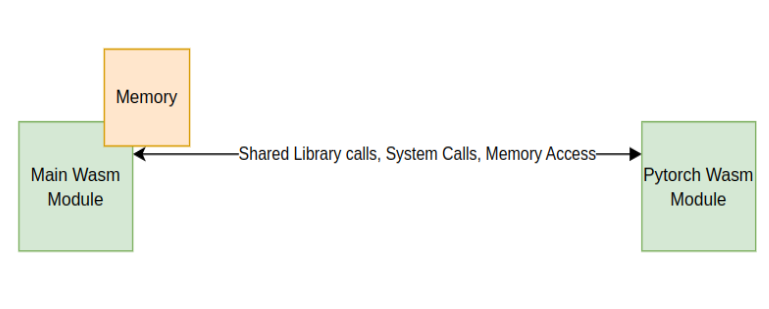
\includegraphics[width=1.0\textwidth]{Images/dynamic-linking-arch.png}
\caption{Architecture for remote module execution with shared memory.}
\label{fig:dynamic-linking-arch}
\end{figure}


\subsection{Remote Module Execution with Component Model and wRPC}
\label{optimized-solution}
The second solution represented in Figure \ref{fig:architecture}, builds on the Component Model and wRPC, by enforcing \textbf{shared-nothing} principles and leveraging the immutable high-level WIT interfaces from the component model, this approach eliminates the need of sharing memory between the components.

\begin{itemize}
\item Components communicate explicitly via immutable WIT interfaces, and each component has it's own linear memory.
\item Remote execution is enabled through wRPC
\end{itemize}

\begin{figure}[h!]
\centering
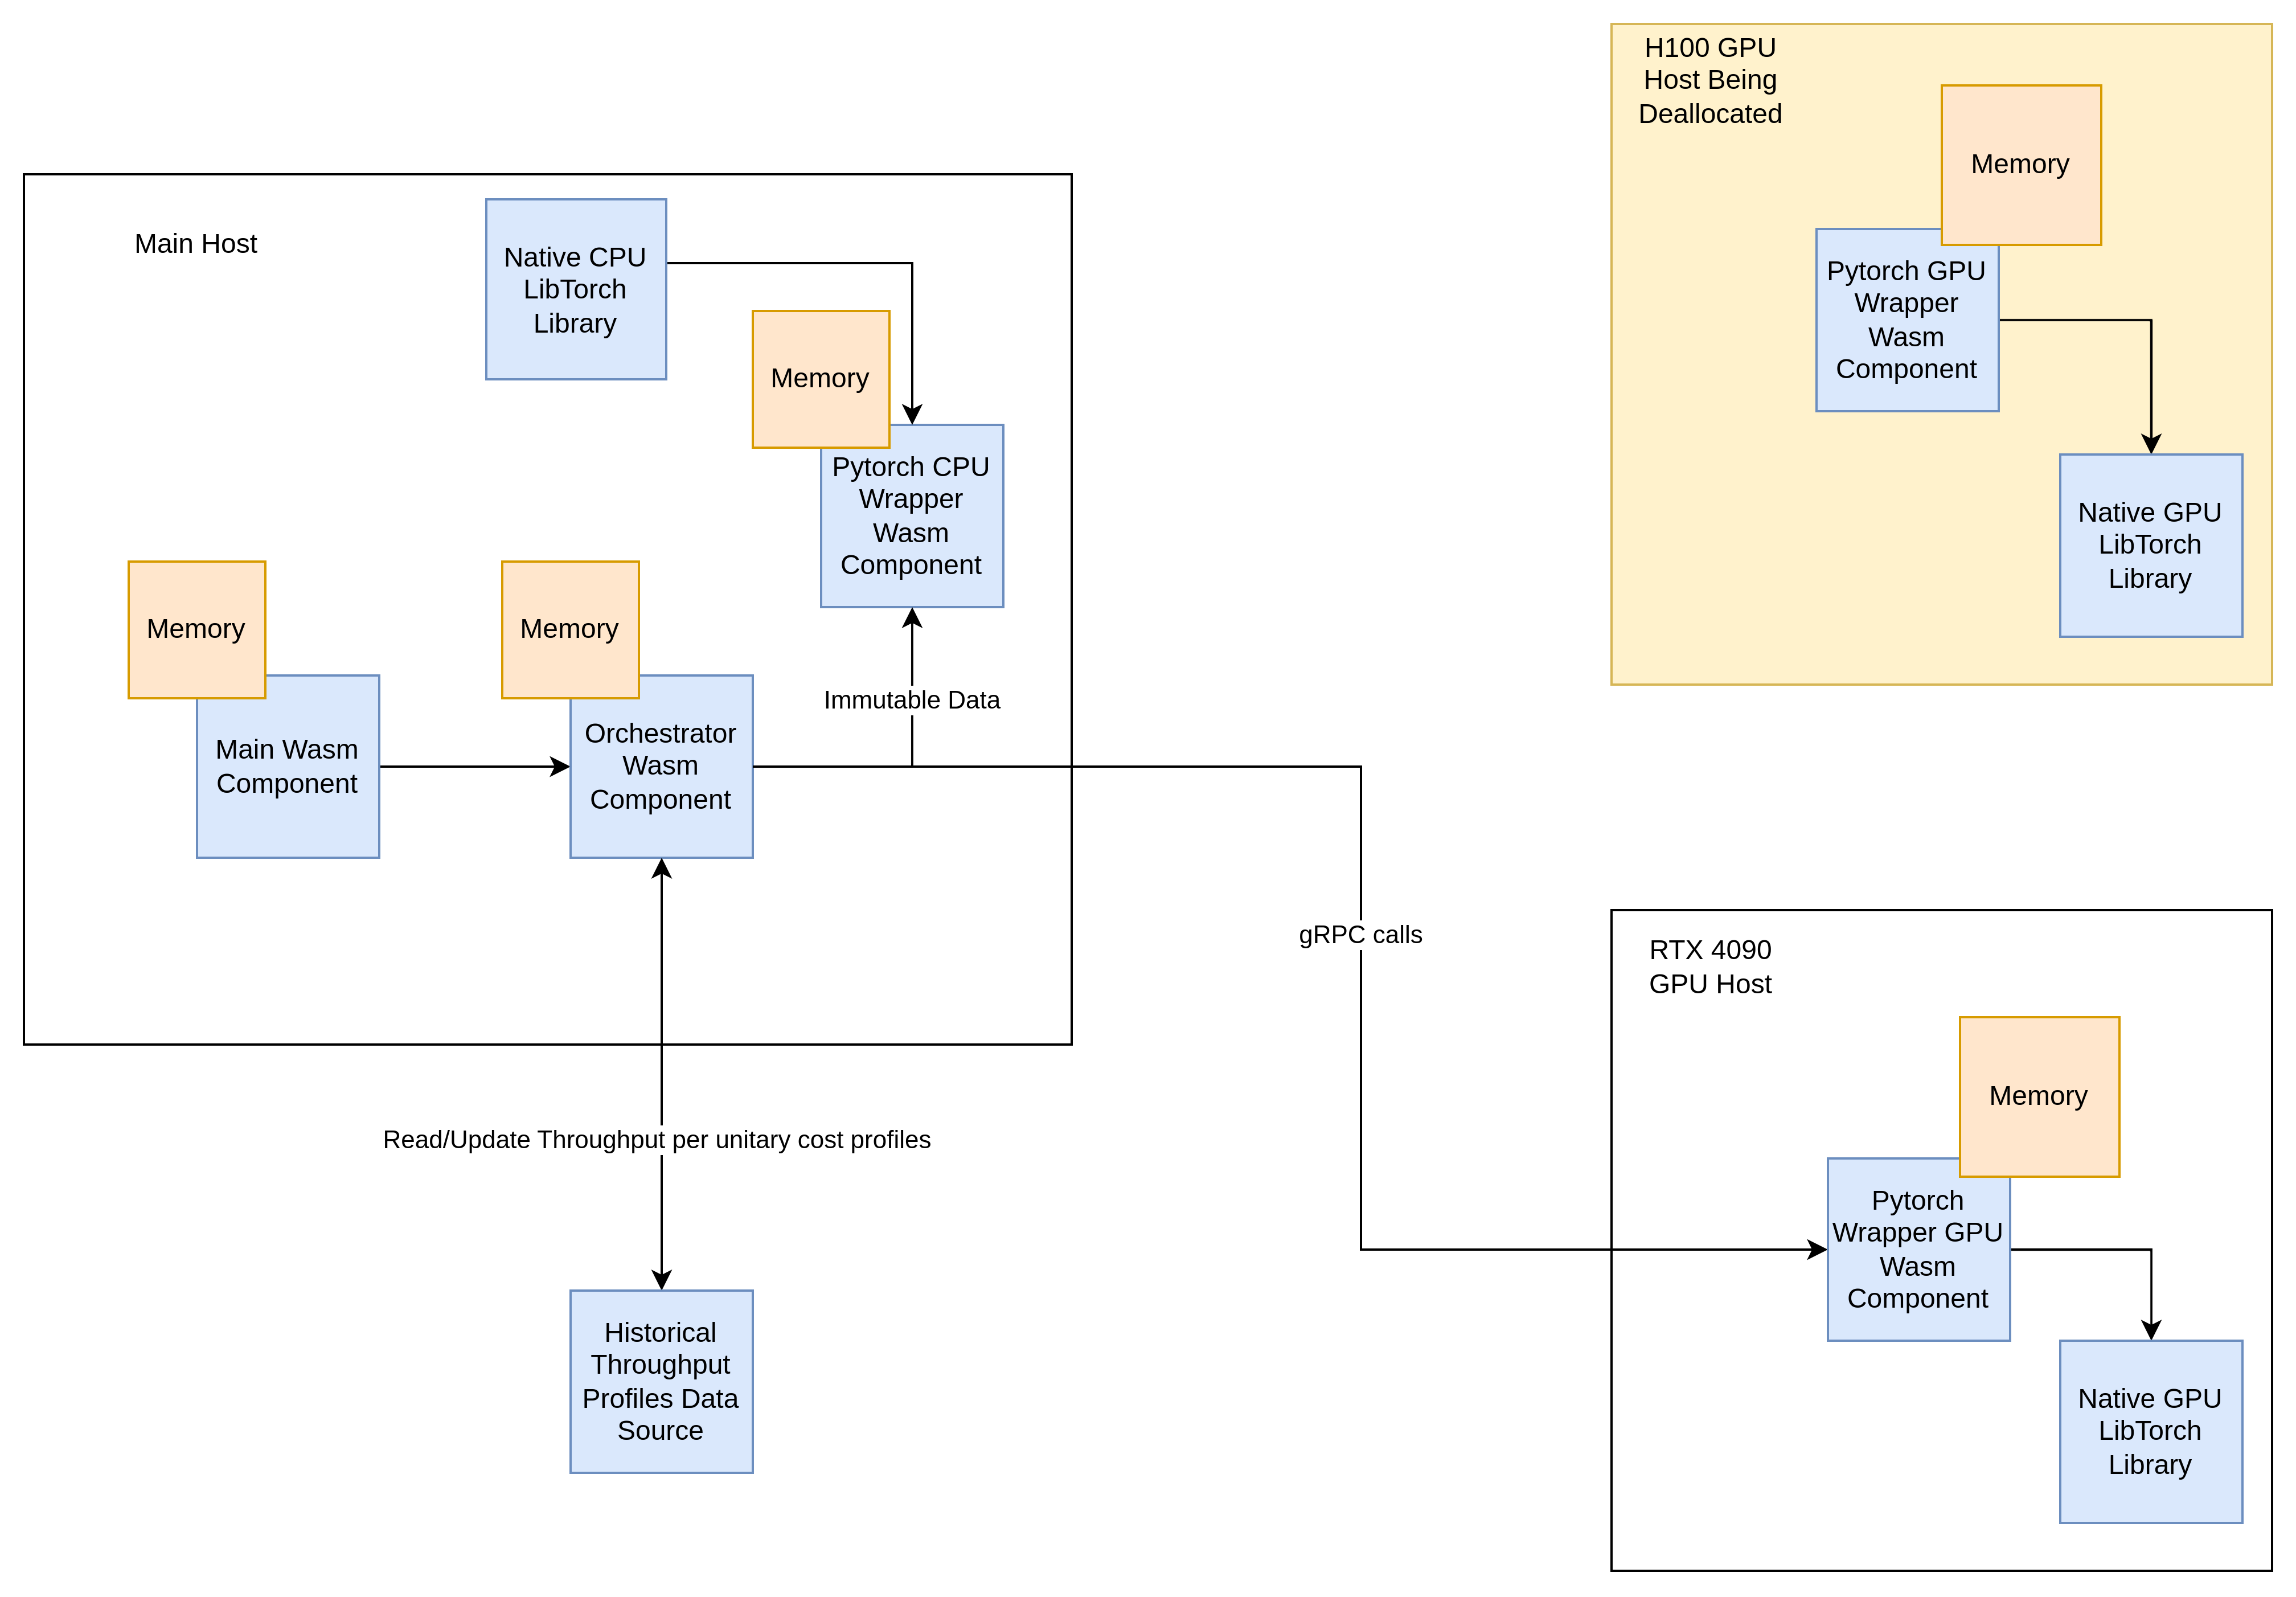
\includegraphics[width=1.0\textwidth]{Images/component-model-arch.png}
\caption{System architecture for dynamic selection of accelerators based on workload. }
\label{fig:architecture}
\end{figure}


\textbf{Steps for implementation}:
\begin{enumerate}
\item Compile shared libraries and main modules as WebAssembly components.
\item Use wRPC to establish communication between components.
\item Dynamically load components at runtime and resolve their interfaces.
\item Enable remote function execution using wRPC across distributed environments.
\end{enumerate}



By dynamically selecting the appropriate accelerator based on throughput and device utilization, we believe lower costs and possible energy savings can be achieved. 
The use of the standardized WASI v2 infrastructure, which allows interoperability between languages due to the WIT interface, flexibility in distributing the components across servers with the wRPC protocol, and not having the performance bottlenecks of the first solution derived from the shared memory, this provides the necessary abstraction to enable this dynamic selection seamlessly.


\pagebreak
% \section{Conclusion}
% We presented two solutions for dynamic linking in WebAssembly. The first, using WASI v1, offers a manual but functional implementation. The second, leveraging the Component Model and wRPC, provides a streamlined and efficient solution that balances performance, isolation, and scalability. These approaches enable dynamic linking and remote execution, paving the way for advanced, flexible, and distributed WebAssembly applications.

%%%%%%%%%%%%%%
% Evaluation %
%%%%%%%%%%%%%%
% \section{Evaluation}


% In this section, we outline our evaluation methodology, describe the metrics used to assess our system, and explain the benchmarks relevant to different aspects of our implementation. The evaluation aims to validate our approach by analyzing cost-performance, energy efficiency, and scalability. Finally, we will discuss the results and draw conclusions about the system's performance.

% \subsection{Evaluation Hypotheses and Expected Outcomes}


% We aim to test our implementation with the following metrics.

% \subsection{Maximization Objectives}

% \begin{itemize}
%     \item \textbf{Throughput per unitary cost:} 
% We aim to demonstrate that throughput per unitary cost spent is higher with our implementation compared to just doing horizontal scaling of the same hardware type. By varying the number of invocations, inter-arrival time and model size, we can illustrate how our approach achieves a superior cost-performance ratio. 
%     \item \textbf{Throughput per Watt:} 
%     This metric is designed to showcase the energy efficiency of our implementation. By conducting a comparative analysis of the throughput per watt between our system and horizontal scaling of the same hardware type, we aim to analyze possible energy savings.
% \end{itemize}

% \subsection{Minimization Objectives}

% \begin{itemize}
%     \item \textbf{Latency by Varying Number of Invocations:} 
% We analyze how latency changes as the number of invocations varies, thereby demonstrating the scalability of our system without compromising response time. 
%     \item \textbf{Latency by Varying Model Size:} 
% This metric evaluates how the latency is impacted by the size of the model being used. It helps to analyse how model size affects latency specially when loading it's weights to the GPUs.
% \end{itemize}

% \subsection{Summary}
% With these evaluations, we aim to demonstrate that our implementation will provide lower cost, higher energy savings while maintaining latency constraints.

\section{Evaluation}

In this section, we outline our evaluation methodology, describe the evaluation hypotheses, define the metrics used to assess our system and the evaluation environment. 

\subsection{Evaluation Plan}

To validate our implementation, we will use metrics that measure cost-effectiveness, energy efficiency, and latency under various workloads. The experiments will involve varying the number of invocations, inter-arrival times, and model sizes to simulate diverse usage scenarios. 

\subsection{Evaluation Hypotheses and Expected Outcomes}

The evaluation aims to validate the following hypotheses:
\begin{itemize}
    \item \textbf{Does our system achieve high throughput per unitary cost compared to only doing horizontal scaling?}
        \begin{itemize}
        \item \textbf{Expected Outcome:} Our system is expected to deliver higher throughput per unitary cost by optimizing hardware usage through heterogeneous vertical scaling.
    \end{itemize}
    \item \textbf{Does our system achieve high throughput per watt compared to horizontal scaling?}: 
        \begin{itemize}
        \item \textbf{Expected Outcome:} We anticipate achieving higher throughput per watt due to the heterogeneous vertical scaling.
    \end{itemize}
    \item \textbf{How does the system perform in terms of latency as the number of invocations and model sizes increase?}
    \begin{itemize}
        \item \textbf{Expected Outcome:} The system maintains low latency under increased invocation rates and larger model sizes, showcasing scalability without significant degradation in response time.
    \end{itemize}

\end{itemize}

\subsection{Evaluation Metrics}

We will use the following metrics to assess the performance of our implementation:
\begin{itemize}
    \item \textbf{Throughput per Unitary Cost}: This metric measures cost-performance efficiency. By comparing throughput per unitary cost spent between our implementation and horizontal scaling, we aim to demonstrate the cost benefits of our heterogeneous resource allocation mechanism.
    \item \textbf{Throughput per Watt}: This metric evaluates energy efficiency. By analyzing throughput per watt under different workloads, we aim to highlight the potential energy savings of our system compared to homogeneous scaling.
    \item \textbf{Latency}: This metric assesses the system’s scalability and responsiveness under varying workloads:
    \begin{itemize}
        \item \textbf{Latency by Number of Invocations}: Measures how latency scales with an increasing number of invocations.
        \item \textbf{Latency by Model Size}: Evaluates how the size of the model impacts latency, particularly during weight loading to GPUs.
    \end{itemize}
\end{itemize}

\subsection{Evaluation environment}

For evaluation, we aim to use rented VMs from Vast.AI, which provides an API to rent hosts at an hourly rate with various levels of hardware types, from RTX 4090 to H100's. The hourly rate will be used by the orchestrator to update the throughput per unitary cost profiles in the data source.

\subsection{Evaluation Workload}

We aim to have workloads that reflect real world traces, for this we will create a synthetic dataset with similar inference load distribution over the day compare to the Azure LLM inference trace 2024 open source traces dataset from the DynamoLLM \cite{dynamollm} paper. We will have to create our own synthetic data due to the existing dataset not including the prompt requests due to privacy concerns. Regarding the models we will use various open source LLMs such as the Meta-Llama-3-8B \cite{llama3}.

\subsection{Summary}

With these evaluations, we aim to demonstrate that our implementation will provide lower cost, higher energy savings while maintaining latency constraints.

% For evaluation, we aim to test our implementation with the following metrics:

% and maximize the following:

% throughput per unitary cost with our implementation vs single hardware type scaling

% With this metric, we aim to show that the throughput per unitary cost spent is higher with our implementation compared to scaling smaller hardware such as an RTX 4090.
% To plot this we increase the number of invocations and the

% throughput per watt with our implementation vs single hardware type scaling

% With this metric, we aim to show that the throughput per watt spent is higher with our implementation compared to scaling smaller hardware such as an RTX 4090.

% We aim to minimize the following:

% latency by varying number of invocations
% latency by model size
% latency by inter arrival time

% With this, we aim to show that our implementation does not only take into account the cost benefit and energy saving portion, but also the latency of the invocations via dynamically renting GPU's closest to the users.


% \textbf{Important:} scientific work should be reproducible! 
% When applicable, you are strongly encouraged to create a replication package that follows the open science policies as adopted by SIGSOFT (see \url{https://github.com/acmsigsoft/open-science-policies}).

% \medskip

% \lipsum[2-3]

% Figure \ref{fig:CodeJava} shows a Java code snippet example.

% \begin{figure}
%     \centering
%     \begin{lstlisting}[language=Java]
%         private void adjustRowHeights(Jtable table) {
%             for(int row = num; row < table.getRowCount(); row++) {
%                 int rowHeight = table.getRowHeight();
%                 for(int column = num; column < table.getColumnCount(); column++) {
%                     component comp = table.prepareenderer(table.getCellenderer(row, column), row, column);
%                     rowHeight = math.max(rowHeight, comp.getPreferredSize().height);
%                 }
%                 table.setRowHeight(row, rowHeight);
%             }
%         }
%     \end{lstlisting}
%     \caption{Java code snippet.}
%     \label{fig:CodeJava}
% \end{figure}


% Figure \ref{fig:CodePython} shows an example of a Python code snippet imported from a file.

% \begin{figure}
%     \centering
%     \lstinputlisting[language=Python]{Tables_and_code/code.py}
%     \caption{Python code snippet.}
%     \label{fig:CodePython}
% \end{figure}


%%%%%%%%%%%%%%%%%
% Work Schedule %
%%%%%%%%%%%%%%%%%
\section{Work Schedule}
Our proposed work schedule is available in Figure~\ref{ganttchart}.

\begin{figure}
\centering
\rotatebox{90}{
\tikzset{every picture/.style={xscale=0.8,yscale=0.8,transform shape}}
\begin{ganttchart}[ y unit chart = 0.7cm,
                    vgrid, 
                    bar top shift=-0.1, 
                    bar height=0.6, 
                    title height=0.7]{1}{36}
  \gantttitle{Feb'19}{4}
  \gantttitle{Mar'19}{4}
  \gantttitle{Apr'19}{4}
  \gantttitle{May'19}{4} 
  \gantttitle{Jun'19}{4} 
  \gantttitle{Jul'19}{4} 
  \gantttitle{Aug'19}{4} 
  \gantttitle{Sep'19}{4} 
  \gantttitle{Oct'19}{4} \\
  \gantttitlelist{1,...,4}{1}
  \gantttitlelist{1,...,4}{1}
  \gantttitlelist{1,...,4}{1}
  \gantttitlelist{1,...,4}{1}
  \gantttitlelist{1,...,4}{1}
  \gantttitlelist{1,...,4}{1}
  \gantttitlelist{1,...,4}{1}
  \gantttitlelist{1,...,4}{1}
  \gantttitlelist{1,...,4}{1} \\
  
\ganttgroup{Collect data on Heterogenous Hardware}{1}{7} \\
\ganttbar{Obtain data regarding cost-benefit analysis}{1}{5} \\
\ganttbar{Select architecture details}{6}{7} \\

\ganttgroup{Implementation}{6}{18} \\
\ganttbar{Basic Proxy Implementation}{6}{11} \\
\ganttbar{State Switching Implementation}{12}{18} \\


\ganttgroup{Experimental evaluation}{19}{22} \\
\ganttbar{Run benchmarks and analyze metrics}{19}{20} \\
\ganttbar{Evaluate Solution}{21}{22} \\

\ganttgroup{Writing dissertation}{4}{36} \\
\ganttbar{Alpha version}{4}{24} \\
\ganttbar{Final revision by advisor}{25}{27} \\
\ganttbar{Beta version}{28}{36} \\

\end{ganttchart}
}


\caption{Planned Schedule}
\label{ganttchart}
\end{figure}


%%%%%%%%%%%%%%%%
% BIBLIOGRAPHY %
%%%%%%%%%%%%%%%%
\clearpage
% add Bibliography to TOC
\addcontentsline{toc}{section}{\refname}
% The following command resets the 'emphasis' style for bibliography entries
\normalem
% Name of your BiBTeX file
\bibliography{./Bibliography} % <-- ACTION: Put here your own filename or edit Bibliography.bib to add your references
% The following command modifies the 'emphasis' style for bibliography entries
\ULforem


%%%%%%%%%%%%
% APPENDIX %
%%%%%%%%%%%%
% \clearpage % <-- ACTION: Comment the following blocks if you dont need appendixes
% \appendix
% \input{Sections/AppendixA.tex}

%%%%%%%%%%%%%
%    END    %
%%%%%%%%%%%%%

\end{document}
